%%%%%%%%%%%%%%%%%%%%%%%%%%%%%%%%%%%%%%%%%%%%%%%%%%%%%%%%%%%%%%%%%%%%%%%%%%%%%%
%  PortfolioIQ --- IEEE conference paper
%
%  Build:  latexmk -pdf paper.tex
%  Layout: IEEEtran [conference], double column, 10pt
%
%  Structure follows the department template:
%    Abstract / I Introduction / II Literature Survey / III Methodology /
%    IV Implementation and Result / V Conclusion
%
%  Every numeric claim is reproduced by scripts/reproduce.py under the pinned
%  environment (scikit-learn 1.7.2, numpy 2.2.6, pandas 2.3.3).
%%%%%%%%%%%%%%%%%%%%%%%%%%%%%%%%%%%%%%%%%%%%%%%%%%%%%%%%%%%%%%%%%%%%%%%%%%%%%%
\documentclass[conference]{IEEEtran}
\IEEEoverridecommandlockouts

\usepackage{cite}
\usepackage{amsmath,amssymb,amsfonts}
\usepackage{algorithmic}
\usepackage{graphicx}
\usepackage{float}
\usepackage{booktabs}
\usepackage{multirow}
\usepackage{textcomp}
\usepackage{xcolor}
\usepackage{tikz}
\usetikzlibrary{arrows.meta,positioning,calc}

\usepackage[hyphens]{url}
\Urlmuskip=0mu plus 1mu\relax
\sloppy

% Compact spacing to fit the 6-page limit; no content is affected.
\setlength{\textfloatsep}{5pt plus 2pt minus 2pt}
\setlength{\floatsep}{3pt plus 1pt minus 1pt}
\setlength{\intextsep}{5pt plus 2pt minus 2pt}
\setlength{\abovecaptionskip}{3pt}
\setlength{\belowcaptionskip}{2pt}

\graphicspath{{figures/}}

\begin{document}

\title{Federated Learning-Based Portfolio Rebalancing\\
Necessity Detection}

\author{
    \centering
    \IEEEauthorblockN{
        \footnotesize\begin{tabular}{cc}
            C S Vaishakh & Lakshmy Rajeev \\
            \textit{Department of Artificial Intelligence and Data Science} &
            \textit{Department of Artificial Intelligence and Data Science} \\
            \textit{St. Joseph's College of Engineering \& Technology, Palai} &
            \textit{St. Joseph's College of Engineering \& Technology, Palai} \\
            Choondacherry P.O., Kottayam District, Kerala State -- 686579 &
            Choondacherry P.O., Kottayam District, Kerala State -- 686579 \\
            csvaishakh2027@ai.sjcetpalai.ac.in & lakshmy0004@gmail.com
        \end{tabular}
    }

    \vspace{0.4cm}

    \IEEEauthorblockN{
        \footnotesize\begin{tabular}{cc}
            Rahul Sarang & Sooraj P S \\
            \textit{Department of Artificial Intelligence and Data Science} &
            \textit{Department of Artificial Intelligence and Data Science} \\
            \textit{St. Joseph's College of Engineering \& Technology, Palai} &
            \textit{St. Joseph's College of Engineering \& Technology, Palai} \\
            Choondacherry P.O., Kottayam District, Kerala State -- 686579 &
            Choondacherry P.O., Kottayam District, Kerala State -- 686579 \\
            ars.rahul.san@gmail.com & pssooraj88@gmail.com
        \end{tabular}
    }

    \vspace{0.4cm}

    \IEEEauthorblockN{
        \footnotesize\begin{tabular}{c}
            Saritha M S \\
            \textit{Department of Artificial Intelligence and Data Science} \\
            \textit{St. Joseph's College of Engineering \& Technology, Palai} \\
            Choondacherry P.O., Kottayam District, Kerala State -- 686579 \\
            sarithams123@gmail.com
        \end{tabular}
    }
}

\maketitle

\begin{abstract}
Portfolio rebalancing is usually governed by fixed calendar or drift-band rules
that ignore the market state in which the decision is taken, and the machine
learning systems proposed to replace those rules are commonly trained on labels
emitted by the very heuristics they are meant to supersede. Because such a label
is a deterministic function of the input features, the resulting classifier
recovers the rule rather than the decision, an effect this paper names rule-oracle
degeneracy and measures directly. We present a federated learning-based system
that treats rebalancing as binary necessity detection over a versioned twelve
feature portfolio and market contract, labelled by the sign of a 21-trading-day,
net-of-cost certainty-equivalent gain evaluated over 3{,}706 NIFTY~50 sessions
spanning 2011 to 2026. Detection and federation are developed as equal parts of
one design: a logistic detector whose parameters are a twelve-element weight
vector, and a sample-weighted federated averaging protocol with $L_2$-clipped
updates, contract gating and atomic activation, in which model updates rather
than holdings leave the client. The detector attains a test ROC-AUC of 0.6489
(five-fold cross-validation $0.6519 \pm 0.0094$) with an expected calibration
error of 0.0214. Relabelling the identical 30{,}000 states with the project's own
heuristic, changing nothing but the label function, raises test ROC-AUC to 0.9890,
a gap of 0.3401 attributable to the label and not to the learner, across which the
correlation between elapsed time and the label rises from 0.0256 to 0.6074. That
heuristic predicts realised net-of-cost benefit at 0.5278, and calendar and band
rules at 0.5167 and 0.5146, all close to chance. The aggregation path is
implemented and unit-tested but disabled by default and not experimentally
evaluated here, and no privacy guarantee is claimed.
\end{abstract}

\begin{IEEEkeywords}
portfolio rebalancing, necessity detection, federated learning, federated
averaging, logistic regression, model calibration, NIFTY 50
\end{IEEEkeywords}

%%%%%%%%%%%%%%%%%%%%%%%%%%%%%%%%%%%%%%%%%%%%%%%%%%%%%%%%%%%%%%%%%%%%%%%%%%%%%%
%  Compressed toward the 6-page conference limit (builds at 7 pages): 3
%  figures, 4 tables, 7 core equations. Tables t1_dataset, t3_profiles,
%  t4_generator, t5_hyperparams, t9_ablations, t10_fedavg, t12_statistical,
%  t13_threshold and figures f2_generation, f3_label, f4_label_balance,
%  f5_feature_corr, f6_roc, f7_pr, f8_calibration, f9_corr_heatmap,
%  f10_coefficients, f13_aggregation, f14_cv_folds remain in the repository as
%  supplementary detail; their content is merged into the surviving floats or
%  condensed to prose. See compression_plan.md.
%%%%%%%%%%%%%%%%%%%%%%%%%%%%%%%%%%%%%%%%%%%%%%%%%%%%%%%%%%%%%%%%%%%%%%%%%%%%%%
\section{Introduction}
\label{sec:introduction}

A portfolio left untouched does not stay where it was put: differential asset
returns drift realised weights away from the risk--return position that was
chosen~\cite{markowitz1952,sharpe1966}. Rebalancing restores that position, but
every restoration pays spread, brokerage and impact costs and liquidates
positions whose recent strength may persist~\cite{jegadeesh1993}, so the
decision is a cost--benefit test on the current drift, market state and
transaction cost jointly. Incumbent practice answers with rules that use almost
none of this information: calendar rebalancing acts on a fixed interval and
drift-band rebalancing on a fixed threshold, both blind to the volatility,
drawdown and trend that determine whether a round trip is worth its price. The
applied literature argues this conceptually rather than measuring
it~\cite{adedoyin_ai,kumari2024}; measured against forward, net-of-cost outcomes
on our data, a 90-day calendar rule and a drift-band rule attain test AUC
$0.5167$ and $0.5146$, both close to chance. Fig.~\ref{fig:f1} shows the
system in which we replace such a rule with a learned detector.

The data this decision needs cannot reasonably be centralised: holdings
disclose wealth, leverage and trading history and remain identifying long
after any label is stripped, while a single participant produces too few
rebalancing states to learn a market-wide regularity alone. Federated
averaging resolves this cleanly for a linear detector, since its
parameters --- a twelve-element weight vector and intercept --- are exactly
the object federated averaging is defined over~\cite{mcmahan2017}, needing no
distillation step. Transmitting updates instead of holdings is data
minimisation, not a privacy guarantee; no differential privacy or secure
aggregation is implemented anywhere in this paper.

Supervised rebalancing has no naturally observable label, and the expedient
response is to label historical states with the output of the very heuristic
the model should replace. We call the resulting pathology \emph{rule-oracle
degeneracy}: the label is a deterministic function of the features the rule
reads, so the classifier decompiles the rule instead of learning an economic
decision. Section~\ref{sec:implementation} shows this is large enough to be
mistaken for success: on one fixed corpus, holding everything but the label
function constant, the same pipeline reaches test AUC $0.9890$ against
heuristic labels and $0.6489$ against a forward, net-of-cost backtest.

\subsection{Contributions}
\begin{itemize}
\item \textbf{C1: Backtest-derived labels for rebalancing-necessity detection.}
Each label is the sign of a forward 21-trading-day, net-of-cost
certainty-equivalent gain (Section~\ref{sec:methodology}), evaluated on
$3{,}706$ NIFTY~50 sessions (2011-08-01--2026-07-31) at $0.35\%$ round-trip
cost, over $30{,}000$ generated states with structural positive rate $0.5009$.
\item \textbf{C2: A quantified measurement of rule-oracle degeneracy.} A
matched control varying only the label function measures a gap of $0.3401$
test AUC attributable to the label, not the learner (Section~\ref{sec:implementation}).
\item \textbf{C3: A hardened federated aggregation protocol.} Updates are
$L_2$-clipped and combined by a sample-weighted mean, gated by a minimum
participant count, an upload cap and a per-account throttle, with atomic
activation. It is implemented and unit-tested but disabled by default and not
experimentally evaluated here.
\item \textbf{C4: A cross-runtime parity contract} that pins feature order and
scaler constants by version, so pooling is well defined and mismatched
contracts are rejected rather than averaged, to $10^{-12}$/$10^{-5}$ agreement.
\item \textbf{C5: An explicit model-selection trade.} The linear detector
surrenders $0.0301$ test AUC to a random forest and is chosen anyway because
its parameters are averageable and its probabilities are calibrated (ECE
$0.0214$); the deficit is reported, not suppressed.
\end{itemize}

The evidence is correspondingly narrow: the cross-section is generated rather
than observed, no path-based backtest or federated experiment was run, and
none of this constitutes investment advice. Section~\ref{sec:literature}
surveys the related literature; Section~\ref{sec:methodology} presents
detection and federation as equally weighted halves of one design;
Section~\ref{sec:implementation} reports the results; Section~\ref{sec:conclusion}
concludes.

% F1 --- system architecture (double column)
\begin{figure*}[t]
\centering
\resizebox{0.86\linewidth}{!}{%
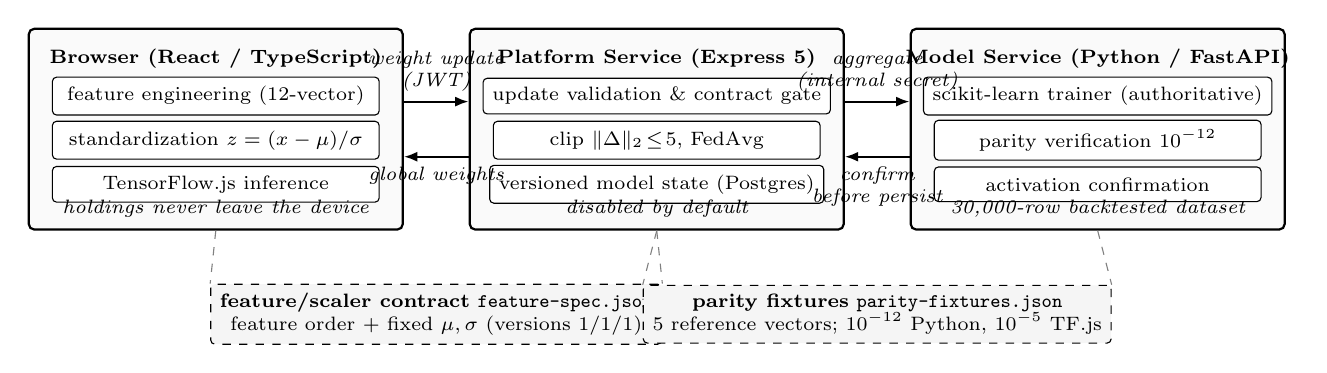
\begin{tikzpicture}[
  font=\footnotesize,
  tier/.style={draw, rounded corners=2pt, thick, minimum height=2.55cm,
               minimum width=4.75cm, align=center, fill=black!2},
  box/.style={draw, rounded corners=1.5pt, minimum width=4.15cm,
              minimum height=0.44cm, align=center, font=\scriptsize, fill=white},
  contract/.style={draw, dashed, rounded corners=1.5pt, align=center,
                   font=\scriptsize, fill=black!4, minimum height=0.72cm},
  flow/.style={-{Latex[length=1.7mm]}, thick},
  lbl/.style={font=\scriptsize\itshape, midway, align=center}
]

% ---- tiers
\node[tier] (browser) at (0,0) {};
\node[tier] (platform) at (5.6,0) {};
\node[tier] (model) at (11.2,0) {};

\node[font=\scriptsize\bfseries, anchor=north] at ([yshift=-1.5mm]browser.north)
  {Browser (React / TypeScript)};
\node[font=\scriptsize\bfseries, anchor=north] at ([yshift=-1.5mm]platform.north)
  {Platform Service (Express 5)};
\node[font=\scriptsize\bfseries, anchor=north] at ([yshift=-1.5mm]model.north)
  {Model Service (Python / FastAPI)};

% ---- browser internals
\node[box] (b1) at (0,0.42) {feature engineering (12-vector)};
\node[box] (b2) at (0,-0.14) {standardization $z=(x-\mu)/\sigma$};
\node[box] (b3) at (0,-0.70) {TensorFlow.js inference};
\node[font=\scriptsize\itshape, anchor=south] at ([yshift=0.5mm]browser.south)
  {holdings never leave the device};

% ---- platform internals
\node[box] (p1) at (5.6,0.42) {update validation \& contract gate};
\node[box] (p2) at (5.6,-0.14) {clip $\lVert\Delta\rVert_2\!\le\!5$, FedAvg};
\node[box] (p3) at (5.6,-0.70) {versioned model state (Postgres)};
\node[font=\scriptsize\itshape, anchor=south] at ([yshift=0.5mm]platform.south)
  {disabled by default};

% ---- model service internals
\node[box] (m1) at (11.2,0.42) {scikit-learn trainer (authoritative)};
\node[box] (m2) at (11.2,-0.14) {parity verification $10^{-12}$};
\node[box] (m3) at (11.2,-0.70) {activation confirmation};
\node[font=\scriptsize\itshape, anchor=south] at ([yshift=0.5mm]model.south)
  {30{,}000-row backtested dataset};

% ---- flows
\draw[flow] ([yshift=3.5mm]browser.east) -- ([yshift=3.5mm]platform.west)
  node[lbl, above]{weight update\\(JWT)};
\draw[flow] ([yshift=-3.5mm]platform.west) -- ([yshift=-3.5mm]browser.east)
  node[lbl, below]{global weights};
\draw[flow] ([yshift=3.5mm]platform.east) -- ([yshift=3.5mm]model.west)
  node[lbl, above]{aggregate\\(internal secret)};
\draw[flow] ([yshift=-3.5mm]model.west) -- ([yshift=-3.5mm]platform.east)
  node[lbl, below]{confirm\\before persist};

% ---- shared contracts
\node[contract] (c1) at (2.8,-2.35)
  {\textbf{feature/scaler contract} \texttt{feature-spec.json}\\
   feature order $+$ fixed $\mu,\sigma$ (versions 1/1/1)};
\node[contract] (c2) at (8.4,-2.35)
  {\textbf{parity fixtures} \texttt{parity-fixtures.json}\\
   5 reference vectors; $10^{-12}$ Python, $10^{-5}$ TF.js};

\draw[dashed, gray] (browser.south) -- (c1.north west);
\draw[dashed, gray] (platform.south) -- (c1.north east);
\draw[dashed, gray] (platform.south) -- (c2.north west);
\draw[dashed, gray] (model.south) -- (c2.north east);

\end{tikzpicture}%
}
\caption{System architecture. Features are computed and standardized in the
browser; the platform validates and aggregates federated updates; the model
service is the authoritative trainer that confirms an aggregate before it is
published. Two versioned contracts keep both runtimes numerically identical. The
federated path is implemented and unit-tested but disabled by default and not
evaluated in this paper.}
\label{fig:f1}
\end{figure*}


\section{Literature Survey}\label{sec:literature}

\textit{Rebalancing policy.} Portfolio construction selects weights that trade
expected return against variance~\cite{markowitz1952}, and risk-adjusted
performance measures make the resulting drift consequential~\cite{sharpe1966}.
Practice answers drift with calendar or threshold rules, neither free of
opportunity cost since restoring target weights trims positions whose
intermediate-horizon returns are reported to continue rather than
revert~\cite{jegadeesh1993}. The applied literature that proposes machine
learning here argues the point conceptually: Adedoyin catalogues the model
families that might replace fixed-interval rebalancing and the overfitting
risk they face~\cite{adedoyin_ai}, and Kumari reaches a similar conclusion for
threshold policies, naming logistic regression as the appropriate device for a
binary financial outcome~\cite{kumari2024}. Both are reviews; neither states a
reproducible method, a labelling procedure or a numeric result, and this work
uses them only as motivation and as precedent for the model class.

\textit{Financial ML and federated mechanics.} Mashrur \emph{et al.} survey
machine learning for financial risk management and establish supervised
classifiers, logistic regression among them, as standard instruments for
binary financial determinations, while also naming generated data and
federated learning as directions for settings where confidential or rare-event
data are unavailable~\cite{mashrur2020}. Deep architectures apply the same
representation-learning spirit to asset universes~\cite{heaton2017}. Neither
models the portfolio-level rebalancing action itself. Federated averaging
trains a shared model by repeatedly averaging local updates instead of
centralising data~\cite{mcmahan2017}, applicable across the horizontal,
vertical and transfer settings surveyed by Yang \emph{et al.}~\cite{yang2019federated};
its dominant obstacle is statistical heterogeneity, which degrades convergence
under non-independent client data~\cite{li2020challenges,li2020noniid}, and
surveys of federated recommendation add that retaining data on-device removes
a class of collection risk while introducing inference and poisoning threats
of its own~\cite{javeed2024}.

\textit{Financial federated evidence.} Noseda \emph{et al.} train a shared
volatility classifier and report federated averaging reaching accuracy close
to centralised training under an IID partition ($0.7162$ vs.\ $0.7295$) and
exceeding isolated local training under a non-IID partition ($0.7206$ vs.\
$0.5366$), while strong differential-privacy noise collapses utility below
every non-private configuration~\cite{noseda2025}. Yu, Wynter and Lim apply
federated reinforcement learning to portfolio management and find that plain
aggregation causes training to fail, motivating a personalised, regularised
server objective~\cite{yu2022fedrl}. The lesson is that collaboration can
approach centralised quality on heterogeneous financial data, but neither
privacy mechanisms nor plain averaging are free of cost.

Table~\ref{tab:t14} positions the present work against this survey. No
identified work treats whether a drifted portfolio requires rebalancing now as
supervised binary classification trained on forward, net-of-cost outcome
labels, and none measures the degeneracy that arises when a rebalancing model
is trained on the labels of the rule it replaces. This paper occupies that
slot: it formulates rebalancing-necessity detection on backtested outcome
labels, quantifies the resulting degeneracy against heuristic labels, and
couples the detector to a federated design exchanging model updates rather
than portfolio records.

% T14 --- literature comparison matrix (double column, Literature Survey)
\begin{table*}[t]
\caption{Positioning of the present work against the surveyed literature}
\label{tab:t14}
\centering
\scriptsize
\setlength{\tabcolsep}{4pt}
\begin{tabular}{@{}llllll@{}}
\toprule
Work & Primary focus & Method & Federated & Label source & Numeric results \\
\midrule
Adedoyin \cite{adedoyin_ai} & Rebalancing & Conceptual, model-agnostic & No & --- & None reported \\
Kumari \cite{kumari2024} & Portfolio management & Conceptual review & No & --- & None reported \\
Mashrur \emph{et al.} \cite{mashrur2020} & Financial risk & Survey (taxonomy) & Named as future work & --- & Survey only \\
Heaton \emph{et al.} \cite{heaton2017} & Portfolio construction & Deep architectures & No & Market returns & Yes \\
Noseda \emph{et al.} \cite{noseda2025} & Volatility forecasting & LSTM with FedAvg & Yes, evaluated & Engineered volatility & Yes \\
Javeed \emph{et al.} \cite{javeed2024} & Recommender privacy & Survey (threat model) & Yes, as subject & --- & Survey only \\
Yu \emph{et al.} \cite{yu2022fedrl} & Portfolio management & Federated reinforcement learning & Yes, evaluated & Reinforcement reward & Yes \\
\midrule
This work & \textbf{Rebalancing necessity} & Logistic detector with FedAvg & Implemented, not evaluated
  & \textbf{Forward net-of-cost outcome} & Yes \\
\bottomrule
\end{tabular}

\vspace{0.5mm}
\raggedright\footnotesize
The two columns that isolate the gap are the last two. No surveyed work poses
rebalancing necessity as a supervised binary decision, and none derives its labels
from a forward, net-of-cost outcome; where labels exist they are engineered
targets or reinforcement rewards. The federated column is reported honestly: the
aggregation path of this work is implemented and unit-tested but is not
experimentally evaluated here, whereas \cite{noseda2025} and \cite{yu2022fedrl}
report federated experiments.
\end{table*}


\section{Methodology}\label{sec:methodology}

This section presents the system in two equally weighted halves: detection
and federation.

\subsection{System and Problem Formulation}

The detector is embedded in the three-tier system of Fig.~\ref{fig:f1}: a
\emph{browser tier} that builds the feature vector and infers locally, a
\emph{platform tier} that holds identity and the aggregation core and never
receives holdings, and a \emph{model tier} that is the single authoritative
trainer. Two versioned contracts hold the tiers together --- a feature/scaler
specification and a set of parity fixtures --- detailed in
Section~\ref{sec:methodology}-E, since they are preconditions for aggregation
rather than incidental engineering. Only a twelve-element coefficient vector,
a scalar intercept and a sample count ever cross a tier boundary.

Let $x\in\mathbb{R}^{12}$ describe a portfolio and its market context on a
decision day. Rebalancing-necessity detection is the binary task
\begin{equation}\label{eq:e1}
\hat{y} = g\bigl(f(x;\theta)\bigr),\qquad y\in\{0,1\},
\end{equation}
where $y=1$ denotes that rebalancing is warranted. This models the
\emph{decision}, not the trade schedule implementing it, which is a separate
deterministic engine outside this scope.

\subsection{Features, Dataset and Labels}

The contract fixes twelve quantities in order: seven portfolio descriptors, one
elapsed-time descriptor and four market descriptors, defined together with
their distribution and univariate association with the label in
Table~\ref{tab:t2}. The vector is assembled in that fixed order and
standardized by shared constants,
\begin{equation}\label{eq:e16}
z_i = (x_i - \mu_i)/\sigma_i \ \ \text{if } \sigma_i \geq 10^{-9}, \ \ \text{else } 0,
\end{equation}
part of the versioned contract rather than fitted per run, since federated
averaging is coherent only when every participant occupies the same input
space. This carries a disclosed defect: the shipped constants derive from a
legacy 5{,}000-row dataset rather than the 30{,}000-row training split used
here (largest discrepancy on \texttt{num\_stocks}, $|\Delta\mu|{=}3.9504$); the
defect is disclosed rather than repaired, and
Section~\ref{sec:implementation} quantifies its cost at $+0.0001$ test AUC.

No public dataset pairs portfolio states with realized rebalancing outcomes,
so the corpus is constructed --- generated data is established practice in
financial machine learning where labelled outcomes are unobtainable
\cite{mashrur2020}. The generator emits $30{,}000$ states under seed
$20260804$; each row is one simulated decision on a real trading day. The
\emph{market leg is real}: NIFTY~50 daily closes over $3{,}706$ sessions
(2011-08-01 to 2026-07-31) supply every return and market feature, while only
the cross-section of holdings is generated from one of six basket profiles
with log-normal target weights and a persistent per-symbol factor loading
$\beta_i\in[0.55,1.55]$. The book drifts over $5$--$170$ trading days by a
real market return plus a systematic, sector and idiosyncratic shock, and
forward returns combine the real forward index move with a regime-dependent
reversion term, stronger under volatility/drawdown stress and weaker in calm
uptrends~\cite{jegadeesh1993}. Persistent loadings keep the market factor from
averaging out, regime-dependence keeps returns from collapsing into a function
of weights alone, and drift is \emph{caused} by elapsed time, so elapsed time
reaches the label only along that causal path; exact constants are in the
repository alongside the reproduction script.

The label is the outcome of a forward, net-of-cost backtest rather than a
rule. Let $t$ be target weights, $w$ the drifted current weights and $f$ the
realized forward returns. The investor compares rebalancing against holding
under a mean-variance objective with transaction costs
\cite{markowitz1952,sharpe1966}, and the label is the sign of the resulting net
certainty-equivalent gain,
\begin{equation}\label{eq:e23}
\begin{aligned}
\Delta\mathrm{CE}(w,t,f) ={}& (t-w)^{\!\top} f
+ A\bigl[\mathrm{Var}(w)-\mathrm{Var}(t)\bigr] \\
&- c\,\lVert t-w \rVert_1,\qquad
y = \mathbf{1}\{\Delta\mathrm{CE} > 0\},
\end{aligned}
\end{equation}
with risk aversion $A{=}45.0$ and round-trip cost $c{=}0.0035$ ($35$ basis
points): a \emph{return gain}, a \emph{risk gain} priced through ex-ante
variance, and an \emph{implementation cost}. Because cost scales with
turnover, \eqref{eq:e23} reproduces no-trade-band behaviour without any band
being coded. Over $30{,}000$ rows it yields a positive rate of $0.5009$
obtained structurally, without resampling. The elapsed-time feature $\tau$ is
deliberately absent from \eqref{eq:e23}; it influences the label only through
the drift it causes, removing the time-collinearity defect of the predecessor
heuristic, which instead scored a sigmoid combination of a logistic function
of $\tau$ and a tiered adjustment on drift, concentration, drawdown, trend and
volatility directly from the feature vector. Because that score is a
deterministic function of the same features the classifier receives, a model
trained on its output recovers the rule rather than the decision; it is used
here solely as a negative control, never as the reported detector's label
source.

\subsection{Detection Model and Training}

The detector is a binary logistic regression on the standardized vector of
\eqref{eq:e16},
\begin{equation}\label{eq:e25}
P(y=1\mid x) = \sigma\bigl(\langle \mathbf{w}, z \rangle + b\bigr), \quad
\hat{y} = \mathbf{1}\{P \geq 0.5\},
\end{equation}
fitted by $L_2$-regularized maximum likelihood ($C{=}1$, lbfgs,
\texttt{max\_iter}$=1000$). The $30{,}000$ rows split
$60/20/20$ by source row order into $18{,}000$/$6{,}000$/$6{,}000$, described as
row-order rather than temporal since the corpus carries no market-time index.

The linear model is a deployment choice, not an accuracy choice: its
coefficients are readable log-odds contributions (Table~\ref{tab:t2}) and are
exactly the object federated averaging operates on --- a weight vector plus
intercept with no architectural ambiguity, unlike a tree ensemble, which
admits no meaningful coordinate-wise mean. Identical arithmetic in both
runtimes is what makes the parity contract testable to $10^{-12}$, and the
objective yields calibrated probabilities for an interface that presents a
probability of need rather than a binary instruction. The accuracy price is
quantified in Section~\ref{sec:implementation}.

\subsection{Federated Protocol and Aggregation}

The parameters of \eqref{eq:e25} are improved across accounts without any
account disclosing its holdings. Fig.~\ref{fig:f12} shows the round lifecycle:
a model is seeded from the reference corpus, distributed to authenticated
clients that refuse a contract mismatch, fitted locally in the browser
(warm-started from the global parameters under Adam, lr $0.05$, batch $32$,
so the local optimum is a displacement of the global model), and uploaded ---
twelve coefficients, an intercept, the sample count $n_k$ and the contract
versions, nothing else --- validated for shape, finiteness and contract match
before storage (mismatches rejected as HTTP 409). This scope is stated
without ambiguity: this path is \textbf{implemented, validated and
unit-tested, but disabled by default in the shipped product and not
experimentally evaluated in this paper} --- no federated accuracy, convergence
or robustness result is claimed, and every number in
Section~\ref{sec:implementation} comes from centralized training. Transmitting
updates instead of holdings is data minimisation, not a privacy guarantee;
neither differential privacy nor secure aggregation is implemented. Both
statements are repeated once in Section~\ref{sec:conclusion}.

Aggregation operates on displacements. Let $W_{\mathrm{g}}$ be the active
global model; each admitted update is expressed as a delta and clipped in
$L_2$ norm,
\begin{equation}\label{eq:e28}
\Delta_k = W_k - W_{\mathrm{g}}, \qquad
\tilde{W}_k = W_{\mathrm{g}} + \Delta_k \min\!\left(1,\ \tfrac{L}{\lVert \Delta_k \rVert_2}\right),
\end{equation}
with $L{=}5.0$, then combined by a sample-weighted mean~\cite{mcmahan2017},
\begin{equation}\label{eq:e29}
\bar{W} = \sum_k \frac{n_k}{\sum_j n_j}\, \tilde{W}_k .
\end{equation}
Weighting is not cosmetic: two participants contributing $0.4$ on $120$
samples and $0.8$ on $360$ samples aggregate to $(120\cdot0.4+360\cdot0.8)/480=0.7$
under \eqref{eq:e29}, against $0.6$ unweighted. A round executes only under
\begin{equation}\label{eq:e30}
\bigl|\{k : k \text{ valid}\}\bigr| \geq 2 \ \wedge \ \text{contract versions current},
\end{equation}
since a single participant would publish its local model as the global one,
and mixed contracts would average coefficients defined over different feature
or scaler spaces into a vector that is arithmetically well formed and
semantically meaningless. Heterogeneous client distributions are a known
source of degradation for this family of algorithms
\cite{li2020challenges,li2020noniid}; which regime this system falls into is an
open question, not a claim made here.

\subsection{Robustness and Parity Contract}

The assumed adversary is a participating account, or colluding accounts,
attempting to move the global model; the design assumes neither honest
participants nor cryptographic identity, so it bounds what an identity is
worth rather than preventing Sybil creation: clipping in~\eqref{eq:e28} bounds
any single displacement to $L{=}5.0$ regardless of submitted magnitude, a cap
of $n_k\leq10{,}000$ bounds the weight one identity can claim
in~\eqref{eq:e29} (since $n_k$ is self-reported and unverifiable without
seeing data the design is built not to see), and an hourly throttle bounds
both submission rate and reconnaissance. Aggregation is
administrator-authenticated and lock-protected, activation is
push-before-persist and atomic with the ledger, and the append-only ledger
makes recovery a forward operation; residual weaknesses (a single static
secret, cleartext transport, non-cryptographic identity) are recorded rather
than mitigated, and discussed in Section~\ref{sec:conclusion}.

Federated averaging across two runtimes presupposes they compute the same
function. Two versioned artefacts enforce this: \texttt{feature-spec.json}
fixes the feature order and constants of~\eqref{eq:e16}; \texttt{parity-fixtures.json}
pins five reference vectors and their expected standardized forms, logits and
probabilities, asserted by both test suites at $10^{-12}$ (float64) and
$10^{-5}$ (browser float32). The platform refuses to store or aggregate any
row whose contract triple differs from the active one (HTTP 409) rather than
risk an aggregate silently polluted by incompatible participants --- which is
also what lets the fixed-constant standardization of~\eqref{eq:e16} stand
despite its disclosed scaler-provenance defect, since a scaler refitted
per-client would invalidate~\eqref{eq:e29} outright.

% T2 --- feature summary with formulas folded in (double column)
\begin{table*}[t]
\caption{The twelve-feature contract: definition, distribution over the 30{,}000-row
dataset, univariate association with the label, and learned coefficient}
\label{tab:t2}
\centering
\scriptsize
\setlength{\tabcolsep}{3pt}
\begin{tabular}{@{}cllrrrrr@{}}
\toprule
\# & Feature & Formula & Mean & Std & $r$ with $y$ & Solo AUC & Coef. \\
\midrule
\multicolumn{8}{@{}l@{}}{\emph{Portfolio block}} \\
1 & \texttt{num\_stocks} & $N$ & 12.9093 & 10.0162 & $-0.0219$ & 0.5235 & $-0.0352$ \\
2 & \texttt{max\_stock\_weight} & $w_{\max}=\max_i w_i$ & 0.2705 & 0.2287 & $+0.0291$ & 0.5274 & $+0.0525$ \\
3 & \texttt{top3\_concentration} & $C_3=\sum_{\mathrm{top3}} w_i$ & 0.5253 & 0.3102 & $+0.0216$ & 0.5273 & $-0.1686$ \\
4 & \texttt{total\_weight\_drift} & $D_{\mathrm{ew}}=\sum_i|w_i-\tfrac1N|$ & 0.4092 & 0.3433 & $+0.0331$ & 0.5321 & $+0.0411$ \\
5 & \texttt{portfolio\_return} & $R_p=\sum_i w_iR_i$ & 0.0570 & 0.1099 & $+0.1979$ & 0.6051 & $+1.0661$ \\
6 & \texttt{portfolio\_volatility} & $V_p=\sum_i w_i(R_i{-}R_p)^2$ & 0.0106 & 0.0209 & $+0.0869$ & 0.5651 & $-0.0213$ \\
7 & \texttt{sector\_concentration} & $S=\max_s\sum_{i\in s} w_i$ & 0.4386 & 0.2759 & $+0.0239$ & 0.5170 & $+0.0645$ \\
8 & \texttt{days\_since\_last\_rebalance} & $\tau$ (calendar days) & 122.6721 & 67.2327 & $+0.0256$ & 0.5157 & $-0.0978$ \\
\midrule
\multicolumn{8}{@{}l@{}}{\emph{Market block}} \\
9 & \texttt{market\_return\_30d} & $m_{30}=\mathrm{Cl}_t/\mathrm{Cl}_{t-30}-1$ & 0.0144 & 0.0555 & $+0.0441$ & 0.5417 & $+0.0894$ \\
10 & \texttt{market\_volatility\_30d} & $\sigma_m=\mathrm{std}_{30}(r)$ & 0.0090 & 0.0047 & $+0.1086$ & 0.5975 & $+1.0835$ \\
11 & \texttt{market\_drawdown\_90d} & $\delta_{90}=(\mathrm{Cl}_t{-}H_{90})/H_{90}$ & $-0.0411$ & 0.0480 & $-0.0095$ & 0.4972 & $-0.2602$ \\
12 & \texttt{market\_trend} & $\mathbf{1}\{\mathrm{MA}_{20}{>}\mathrm{MA}_{50}\}$ & 0.6733 & 0.4690 & $+0.0096$ & 0.5090 & $-0.0941$ \\
\bottomrule
\end{tabular}

\vspace{0.5mm}
\raggedright\scriptsize
$w_i=q_iP_i/\sum_j q_jP_j$; $R_i=(P_i-P_i^0)/P_i^0$; $\mathrm{Cl}[\cdot]$ are
index closes, $r_t=\mathrm{Cl}[t]/\mathrm{Cl}[t-1]-1$, $H_{90}$ the 90-session
peak. Solo AUC: logistic fit on that feature alone. Coefficients: standardized
units, intercept $1.6694$; the shipped scaler is fitted on a legacy 5{,}000-row
set, not this one (Table~\ref{tab:t6}).
\end{table*}

% F12 --- federated aggregation round (single column)
\begin{figure}[tb]
\centering
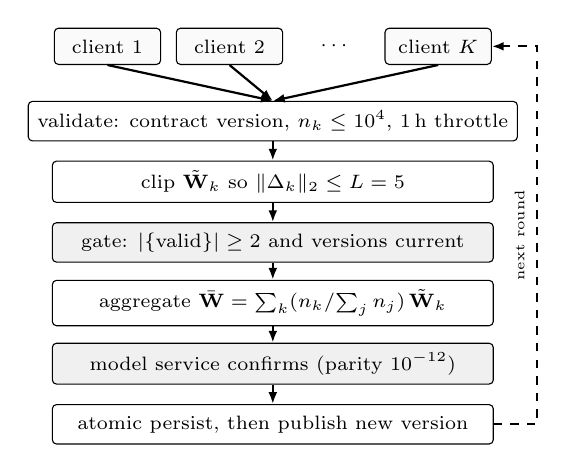
\begin{tikzpicture}[
  font=\scriptsize,
  cl/.style={draw, rounded corners=1.5pt, minimum width=1.35cm,
             minimum height=0.46cm, fill=black!2, align=center},
  st/.style={draw, rounded corners=1.5pt, minimum width=5.6cm,
             minimum height=0.5cm, align=center, fill=white},
  gate/.style={draw, rounded corners=1.5pt, minimum width=5.6cm,
               minimum height=0.5cm, align=center, fill=black!6},
  flow/.style={-{Latex[length=1.5mm]}, thick}
]

\node[cl] (c1) at (-1.9,0) {client 1};
\node[cl] (c2) at (-0.35,0) {client 2};
\node[font=\scriptsize] at (1.0,0) {$\cdots$};
\node[cl] (ck) at (2.3,0) {client $K$};

\node[st] (val) at (0.2,-0.95)
  {validate: contract version, $n_k\le 10^4$, 1\,h throttle};
\node[st] (clip) at (0.2,-1.72)
  {clip $\tilde{\mathbf{W}}_k$ so $\lVert\Delta_k\rVert_2\le L=5$};
\node[gate] (gate) at (0.2,-2.49)
  {gate: $\lvert\{\text{valid}\}\rvert\ge 2$ and versions current};
\node[st] (agg) at (0.2,-3.26)
  {aggregate $\bar{\mathbf{W}}=\sum_k (n_k/\!\sum_j n_j)\,\tilde{\mathbf{W}}_k$};
\node[gate] (conf) at (0.2,-4.03)
  {model service confirms (parity $10^{-12}$)};
\node[st] (pub) at (0.2,-4.80)
  {atomic persist, then publish new version};

\foreach \c in {c1,c2,ck} {\draw[flow] (\c.south) -- (val.north);}
\draw[flow] (val) -- (clip);
\draw[flow] (clip) -- (gate);
\draw[flow] (gate) -- (agg);
\draw[flow] (agg) -- (conf);
\draw[flow] (conf) -- (pub);

\draw[flow, dashed] (pub.east) -- ++(0.55,0) |- (ck.east);
\node[font=\tiny, anchor=west] at (3.15,-2.4) {\rotatebox{90}{next round}};

\end{tikzpicture}
\caption{A federated aggregation round, cf.~\eqref{eq:e28}--\eqref{eq:e30}. Updates
are accepted only on the current contract version, $L_2$-clipped, and persisted
only after the model service confirms the aggregate. Implemented and unit-tested;
disabled by default and not evaluated here.}
\label{fig:f12}
\end{figure}


\section{Implementation and Result}
\label{sec:implementation}

\subsection{Implementation}

The detector of Section~\ref{sec:methodology} is deployed as the three-tier
system of Fig.~\ref{fig:f1}; the evaluation below reproduces the deployed
model service's protocol exactly, under the pinned environment (scikit-learn
1.7.2, numpy 2.2.6, pandas 2.3.3, seed $20260804$), and every value here was
re-executed by a single reproduction script against the committed data. The
primary corpus is $30{,}000$ generated rows, split $60/20/20$ in source-row
order (test positive rate $0.5027$); this is not a temporal split, since the
generator emits no timestamp, and the row-shuffled ablation of
Table~\ref{tab:t6} establishes only that row order introduces no artifact, a
weaker property than a genuine temporal holdout. Features use the shipped
scaler constants, whose legacy provenance defect is disclosed in
Section~\ref{sec:methodology} and whose cost is quantified below.

\subsection{Performance Evaluation}

The primary detector attains test AUC $0.6489$ (validation $0.6585$, indicating
no overfitting) against a chance baseline of $0.5000$ and a majority-class
accuracy of $0.5027$; all other measures (PR-AUC, precision, recall, $F_1$,
MCC, balanced accuracy) are in Table~\ref{tab:t6} and each exceeds its
baseline. The probability output is usable as a probability, at Brier score
$0.2336$ (baseline $0.25$) and expected calibration error $0.0214$ over ten
bins. Five-fold
cross-validation gives AUC $0.6519\pm0.0094$ and PR-AUC $0.6452\pm0.0065$, and
a bootstrap over $1{,}000$ test resamples gives a $95\%$ CI of
$[0.6342,0.6622]$ for test AUC, excluding both the majority-class rate and the
random forest's $0.6790$ below, so the margin over chance is not an artifact
of the test split. At the deployed threshold $0.5$, recall is a conservative
$0.5212$; sweeping the threshold trades this against precision as expected
(recall $0.9907$ at $t{=}0.3$, precision $0.7675$ at $t{=}0.7$), so a
deployment with asymmetric costs should choose its operating point rather than
inherit $0.5$.

Table~\ref{tab:t6} compares the primary model with alternatives on the
identical split: regularization strength is inert ($C\in\{0.1,1,10\}$ all give
test AUC $0.6489$), standardization is not (raw features fall to $0.6333$),
and the best measured model is a random forest at $0.6790$, followed by
gradient boosting ($0.6743$) and a calibrated RBF SVM ($0.6702$) --- a
deficit of $0.0301$ AUC that the logistic detector accepts for the
aggregability and calibration argued in Section~\ref{sec:methodology}.

\subsection{Findings and Comparison with Existing Approaches}

The central finding is a matched negative control that varies the label
function and nothing else. The same $30{,}000$ feature rows are relabelled by
the legacy heuristic scoring rule in place of the backtested
certainty-equivalent criterion~\eqref{eq:e23}; rows, features, standardization,
split, model class and evaluation code are identical across both arms.
Fig.~\ref{fig:f11} shows the result: test AUC $0.9890$ under heuristic labels
against $0.6489$ under backtested labels, a gap of $0.3401$ attributable to
the label alone. The mechanism is directly observable: elapsed time correlates
$0.6074$ with the heuristic label, which reads it as an input, and $0.0256$
with the backtested label, which contains no elapsed-time term; the two
labellings agree on only $0.5221$ of rows. The figure $0.9890$ is a degeneracy
exhibit, not an achievement --- it is the score returned when the oracle
scored against is the rule the model was given to imitate --- and $0.6489$ is
the honest difficulty of the task once that oracle is replaced by a forward,
net-of-cost outcome. A separate $5{,}000$-row corpus labelled by the same
heuristic reaches test AUC $0.9310$ and is reported only as corroboration,
since its corpus and class balance differ and the shipped scaler is in-sample
for it.

Table~\ref{tab:t7} scores the conventional policies against outcome labels on
the same test rows. The calendar rule attains AUC $0.5167$, the band trigger
$0.5146$, and --- the argumentative payload --- the legacy heuristic applied
directly as a decision rule attains only $0.5278$: the rule that a naively
supervised model reproduces at $0.9890$ predicts actual net-of-cost benefit
barely above chance, so recovering the rule and deciding well are almost
unrelated objectives. Paired McNemar tests confirm the ordering in both
directions (Table~\ref{tab:t7}): the detector significantly beats every
deterministic rule and the heuristic itself ($p<10^{-16}$ throughout), and is
itself significantly beaten by both tree ensembles. Against the alternative
learners the comparison runs the other way and is reported as measured: the
random forest's $0.0301$ AUC advantage is not within noise, but its
parameters admit no meaningful coordinate-wise average, whereas the linear
model's twelve-weight-plus-intercept vector is precisely what federated
averaging operates on. The trade is worth making only because the federated
path is pursued; were federation abandoned, a non-federated nonlinear model
would be the correct choice on this data.

The fitted coefficients (Table~\ref{tab:t2}) are dominated by
\texttt{market\_volatility\_30d} ($+1.0835$) and \texttt{portfolio\_return}
($+1.0661$), following directly from the structure of~\eqref{eq:e23}, while
\texttt{top3\_concentration} carries a negative coefficient despite a positive
univariate correlation --- the signature of a concentration family correlated
at $0.91$--$0.92$. No economic reading is claimed for the small coefficients.

One caveat applies throughout: $0.6489$ is the honest difficulty of the task
under outcome labels, not a ceiling --- no Bayes-rate estimate was computed, and
Table~\ref{tab:t6} already shows nonlinear learners exceeding it, so the claim
is task hardness, not optimality. This evaluation reports classification
metrics only: no path-based backtest was performed, so no Sharpe ratio,
Sortino ratio, maximum drawdown, turnover or annualised return is reported
anywhere in this paper, and no federated experiment was run --- both are
future work.

% T6 --- model comparison merged with ablations
\begin{table}[tb]
\caption{Model comparison and ablations, on the identical split and feature
representation}
\label{tab:t6}
\centering
\scriptsize
\setlength{\tabcolsep}{3pt}
\begin{tabular}{@{}lrrr@{}}
\toprule
Model & Val.\ AUC & Test AUC & Test acc. \\
\midrule
Logistic regression ($C=1$) & 0.6585 & \textbf{0.6489} & 0.6022 \\
Random forest (200, depth 8) & 0.6750 & \textbf{0.6790} & 0.6290 \\
Gradient boosting (200, depth 3) & 0.6729 & 0.6743 & 0.6258 \\
SVM-RBF ($C=1$, calibrated) & 0.6773 & 0.6702 & 0.6173 \\
Logistic regression, raw features & 0.6447 & 0.6333 & 0.5942 \\
Majority-class baseline & --- & 0.5000 & 0.5027 \\
\bottomrule
\end{tabular}

\vspace{1mm}
\begin{tabular}{@{}llrr@{}}
\toprule
& Ablation (vs.\ full 12-feature model, AUC 0.6489) & Test AUC & $\Delta$ \\
\midrule
A1 & without \texttt{days\_since\_last\_rebalance} & 0.6483 & $-0.0006$ \\
A4 & scaler refitted on the training split & 0.6490 & $+0.0001$ \\
\bottomrule
\end{tabular}

\vspace{0.5mm}
\raggedright\footnotesize
Regularization strength is inert ($C\in\{0.1,1,10\}$ all give test AUC
$0.6489$); ensembles use \texttt{random\_state}~$=$~20260804. A1 confirms the
backtested label leaves almost no direct time signal, against the $0.6074$
correlation the same feature exhibits under heuristic labels
(Fig.~\ref{fig:f11}). A4 bounds the disclosed scaler-provenance defect at
$+0.0001$ AUC.
\end{table}

\begin{figure}[tb]
\centering
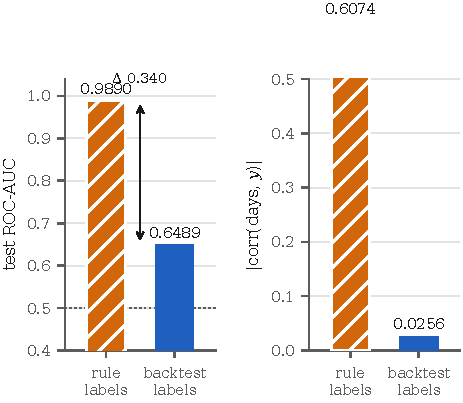
\includegraphics[width=\columnwidth]{f11_negative_control.pdf}
\caption{Rule-oracle degeneracy on one fixed corpus where only the labelling
function varies. Left: heuristic labels give test AUC 0.9890 against 0.6489 for
backtested labels. Right: the elapsed-time/label correlation rises from 0.0256 to
0.6074 across the same substitution. The high left bar is evidence of a
degenerate label, not a capable model.}
\label{fig:f11}
\end{figure}

% T7 --- deterministic baselines and paired significance tests
\begin{table}[tb]
\caption{Deterministic baselines on the same 6{,}000 test rows, and paired
McNemar tests against the logistic detector}
\label{tab:t7}
\centering
\scriptsize
\setlength{\tabcolsep}{3pt}
\begin{tabular}{@{}llrrrrr@{}}
\toprule
& Rule & AUC & Acc. & Prec. & Rec. & MCC \\
\midrule
B0 & always rebalance & 0.5000 & 0.5027 & --- & --- & 0.0000 \\
B1 & $\tau \ge 90$ days & 0.5167 & 0.5175 & 0.5157 & 0.6598 & 0.0349 \\
B2 & band trigger & 0.5146 & 0.5137 & 0.5257 & 0.3319 & 0.0315 \\
B3 & legacy heuristic & 0.5278 & 0.5287 & 0.5235 & 0.6953 & 0.0590 \\
B5 & logistic (ours) & \textbf{0.6489} & \textbf{0.6022} & 0.6250 & 0.5212 & 0.2079 \\
\midrule
\multicolumn{7}{@{}l@{}}{\emph{McNemar exact test vs.\ tree ensembles (paired hard labels)}} \\
\multicolumn{2}{@{}l}{Comparison} & $n_{01}$ & $n_{10}$ & \multicolumn{3}{r@{}}{$p$} \\
\multicolumn{2}{@{}l}{ours vs.\ random forest} & 414 & 575 & \multicolumn{3}{r@{}}{$3.42\times10^{-7}$} \\
\multicolumn{2}{@{}l}{ours vs.\ gradient boosting} & 438 & 580 & \multicolumn{3}{r@{}}{$9.60\times10^{-6}$} \\
\bottomrule
\end{tabular}

\vspace{0.5mm}
\raggedright\footnotesize
B2 fires when \texttt{total\_weight\_drift}~$>0.20$ and
\texttt{max\_stock\_weight}~$>0.35$; B3 is the legacy scoring rule of
Section~\ref{sec:methodology}; B1--B3 emit hard decisions, so their AUC equals
balanced accuracy. McNemar tests against B0/B1/B2/B3 give
$p=4.48\times10^{-24}$, $3.43\times10^{-21}$, $2.38\times10^{-25}$,
$3.24\times10^{-17}$ respectively (detector significantly better in all four;
full $n_{01}/n_{10}$ in the reproduction script). $n_{01}$ counts rows the
detector classifies correctly and the comparator does not; $n_{10}$ is the
converse --- the detector is significantly worse than both tree ensembles.
\end{table}


\section{Conclusion}
\label{sec:conclusion}

This paper treated whether a drifted portfolio should be rebalanced now as a
detection problem trained on forward, net-of-cost outcome labels rather than
on the heuristic the detector replaces. The detector was not designed first
and federated afterwards: because holdings cannot reasonably be centralised
and no single participant holds enough decision states, the linear detector
and the aggregation design were developed together with the labelling work.

The central result is a matched-control measurement of rule-oracle
degeneracy: holding the rows, features, scaler, split, model class and
evaluation code identical and varying only the label function, the same
pipeline attains test AUC $0.9890$ under heuristic labels and $0.6489$ under
backtested labels, a gap of $0.3401$ attributable to the label rather than the
learner (Section~\ref{sec:implementation}). Against backtested outcomes the
deterministic policies this work replaces carry little information --- the
heuristic itself predicts realised benefit at only $0.5278$ --- while the
detector is calibrated (ECE $0.0214$) and stable under 5-fold cross-validation
($0.6519\pm0.0094$).

The federated half is a design contribution of equal standing: updates are
$L_2$-clipped and combined by a sample-weighted mean, gated by a minimum
participant count, an upload cap and a per-account throttle, with
contract-version admission and atomic activation, and browser/server
implementations required to agree to $10^{-12}$. This path is implemented and
unit-tested, but it is disabled by default and not experimentally evaluated in
this paper; sharing model updates instead of raw holdings is data
minimisation, and no privacy guarantee is claimed.

The limits of the evidence are stated plainly: the cross-section is generated
rather than observed, so no external validity is claimed; costs are a flat
$35$ basis points with no market impact; the $60/20/20$ split is row order
with no market-regime holdout; no path-based backtest exists, so no Sharpe,
Sortino, drawdown or turnover figure is available; no federated experiment
was run; elapsed time is exact here but would be estimated from transaction
history for a real user; and the dataset generator resides on an unmerged
branch that must ship alongside the reproduction script and pinned
dependencies.

Future work follows directly: outcome-derived labels, a market-regime
holdout, a multi-factor cross-section and a path-based backtest with turnover
and impact modelling would together establish whether the structure learned
here survives outside the generator that produced it, and a federated
simulation over independent and non-independent partitions, extended to
poisoning robustness, should precede any evaluation of differential privacy
or secure aggregation. Nothing in
this paper constitutes investment advice.


%%%%%%%%%%%%%%%%%%%%%%%%%%%%%%%%%%%%%%%%%%%%%%%%%%%%%%%%%%%%%%%%%%%%%%%%%%%%%%
{\scriptsize
\bibliographystyle{IEEEtran}
\bibliography{references}
}

\end{document}
